\section{Methodology}
\label{sec:methodology}

\subsection{Paired Retrieval and Answer Generation}
For each question, the system retrieves two paragraphs from the question's distractor pool and generates a short answer with numbered paragraph citations. Branch A denotes this first answer. The system uses the original question as the query and ranks the concatenated paragraph titles and texts with BM25Okapi \cite{bm25}. Tokenization uses lowercased alphanumeric tokens and a fixed stop-word list. Branch B retains both paragraphs and, when an unused candidate exists, appends the highest-ranking unused paragraph. The second query concatenates the original question, the top-ranked first-round paragraph's title, and its first sentence. The same generator and answer prompt produce a new answer with paragraph citations.

Caching both branches for every question gives the retrieval policies identical candidate answers for direct comparison. Never returns A and Always returns B. Full-context supplies the entire candidate pool in its original order to one answer-generation call. For branch scores $F_{1,A}$ and $F_{1,B}$, the A/B Oracle chooses B if $F_{1,B}>F_{1,A}$ and chooses A otherwise. It bounds the attainable mean answer F1 over those two cached branches. Full-context accesses the entire pool.

\subsection{First-Round Signals}
The entailment input comes from the pinned three-class DeBERTa-v3-large classifier \cite{nlicheckpoint}. The premise concatenates the distinct valid cited paragraphs in citation order, including their titles. The system falls back to the retrieved paragraphs when there are no valid citations. The hypothesis uses the template \textit{The answer to the question \textquotedblleft\{question\}\textquotedblright{} is: \{answer\}.} The classifier processes up to 512 tokens. The gate uses risk $r=1-p_\mathrm{entail}$ from branch A. Concatenation lets the classifier inspect facts that require two paragraphs. An irrelevant paragraph or an omitted hop can still lead to a misleading score.

The second input tests whether the complete title of either first-round paragraph occurs as a contiguous sequence of words in a sentence of the other paragraph. The detector normalizes Unicode and case before token matching. Define $b=0$ when this lexical link is present and $b=1$ when it is absent. When fewer than two usable paragraphs are available, the gate uses the NLI term alone. The feature measures title overlap as a proxy for a bridge entity. Title variants and coreference can evade this test.

\subsection{Fuzzy and Crisp Decision Rules}
For calibrated anchors $\ell<u$, the high-risk membership is
\begin{equation}
  h(r)=\min\{1,\max\{0,(r-\ell)/(u-\ell)\}\}.
\end{equation}
The low-risk membership is $1-h(r)$. Bridge present and bridge absent use binary memberships. For bridge present, the low- and high-risk consequents are $0$ and $1-w$. For bridge absent they are $w$ and $1$. Product weights and a normalized weighted average give the score $s=(1-w)h(r)+wb$. If the bridge input is unavailable, $s=h(r)$. The same-input crisp comparator replaces $h(r)$ with $\mathbf{1}[r\geq(\ell+u)/2]$ and uses the same rule structure. The NLI-only comparator scores with $s=r$.

Fuzzy and crisp select parameters independently over a shared 27-candidate grid. The low and high anchor candidates are empirical dev risk quantiles $\{.10,.25,.40\}$ and $\{.55,.70,.85\}$, with $w\in\{.125,.25,.375\}$. Each candidate selects 100 of 500 dev questions, maximizing summed paired F1 gain, followed by fewer harmed cases, more improved cases, and the fixed grid order. The dev ranking uses descending $s$, descending $r$, ascending SHA-256 of the UTF-8 string \texttt{42:\textless id\textgreater}, and ascending ID. For each policy, the tuple of the 100th dev question defines the locked boundary. All three gates use the same 20\% dev target. At test time each gate applies its boundary independently to each question. The experimental input set comprises the two locked signals.

\subsection{Sentence-Level Supporting Facts}
The same Qwen model makes a separate selection call after answer generation. It receives the question, the generated answer and numbered candidate sentences from the valid cited paragraphs. The valid selections map back to the original title and zero-based sentence index. Unparseable selection JSON yields an empty set. The selector drops invalid IDs and collapses duplicates. Missing valid paragraph citations yield an empty set. Candidate blocks exceeding the context allowance are split while retaining original candidate IDs. The resulting facts are scored with the official sentence-level metric.

\section{Implementation and Experimental Results}
\label{sec:results}

\subsection{Data, Calibration, and Measurement}
The data are bridge questions from the public validation split of HotpotQA in the distractor setting \cite{hotpotqa}. A seed-42 shuffle produced disjoint pilot, dev and held-out sets of 100, 500 and 1,000 IDs. The held-out set contains 998 ten-paragraph pools and one pool each of four and two paragraphs. The two-paragraph item allows no additional candidate. This evaluation uses a held-out subset of public validation data.

The pilot used \texttt{deepseek-chat}. At the selected retrieval budgets, both gold paragraphs were present for 31\% of questions in A and 59\% in B. Pilot answer F1 was .628, .752 and .765 for A, B and the paired Oracle, respectively. B improved 16 answers, tied 82 and degraded 2. The Oracle's .137 gain over A had a paired 95\% interval of [.077,.203]. Four preset go/no-go conditions passed. These required a gain of at least .05, a positive interval lower bound, at least 10\% improved items, and a degraded-to-improved ratio of at most .5. The numerical thresholds were subjective design choices recorded before the pilot. They required meaningful headroom and enough positives to study gating while limiting observed deterioration.

The dev and formal experiments used Qwen2.5-7B-Instruct \cite{qwen} with vLLM 0.8.5 \cite{vllm}, FP16, greedy decoding at temperature 0, a 128-token completion cap, and a 4096-token context limit. The selected Fuzzy anchors were $(.000589,.381527)$ with $w=.375$ and boundary score $.554886$. Crisp selected $(.000589,.007501)$ with $w=.125$ and boundary score $1.0$. The NLI-only risk boundary was $.173124$. Full-precision boundary tuples and model revisions are retained with the run. Offline GPU DeBERTa inference used a batch size of four and at most 512 tokens per example.

The pinned HotpotQA scorer \cite{hotpotscorer} computes normalized answer exact match (EM), token-level answer F1 and supporting-fact F1 (Supp-F1). The gate's positive label is strictly positive $\Delta F_1=F_{1,B}-F_{1,A}$. We define a tie by $\Delta F_1=0$. To estimate uncertainty, we resample 1,000 paired questions with replacement 10,000 times using seed 42 and take the 2.5th and 97.5th percentiles of the mean paired differences. The five comparisons and interval convention were specified before viewing held-out results. Intervals are individual and condition on the locked policies and cached generations.

For cost, all six executable policies processed the same hash-selected 32 test questions at eight concurrent requests after eight dev warmups per policy. Qwen ran on an NVIDIA Tesla T4 with 4 GiB of CPU weight offload. The NLI classifier ran on CPU with four threads and serialized inference because the two models exceeded available GPU memory when loaded together. Timing spans retrieval or context preparation through the last sentence-selection call. A triggered gate requires A, NLI and B. It invokes the fixed two-round retrieval routine, which rebuilds the first-round ranking. Always directly generates B because the rewrite uses the question and retrieved text, so its online path uses one answer call. Reported LLM tokens include the sentence-selector call, when made.

\begin{table}[!t]
\centering
\caption{Held-out quality and re-retrieval (\%, $n=1{,}000$). The three calibrated gates share a 20\% dev target.}
\label{tab:quality}
\footnotesize
\setlength{\tabcolsep}{3.5pt}
\begin{tabular}{lrrrr}
\hline
Policy & Answer F1 & EM & Supp-F1 & Retrieval \\
\hline
Never & 50.85 & 40.10 & 47.51 & 0.0 \\
Always & 57.66 & 46.20 & 52.38 & 100.0 \\
NLI threshold & 53.89 & 42.70 & 50.15 & 21.9 \\
Crisp & 54.36 & 43.00 & 50.22 & 20.9 \\
Fuzzy & 54.42 & 43.20 & 50.24 & 23.0 \\
Full-context & 64.27 & 50.20 & 54.90 & 0.0 \\
A/B Oracle & 60.61 & 49.20 & 51.35 & 12.3 \\
\hline
\end{tabular}
\end{table}

\begin{table}[!t]
\centering
\caption{Real-path cost on 32 shared questions per policy. Token counts include the answer and selector calls.}
\label{tab:cost}
\footnotesize
\setlength{\tabcolsep}{3.5pt}
\begin{tabular}{lrrrr}
\hline
Policy & Mean (s) & P90 (s) & Input & Output \\
\hline
Never & 19.26 & 23.76 & 697.8 & 27.3 \\
Always & 19.13 & 22.56 & 814.7 & 26.4 \\
NLI threshold & 23.32 & 28.87 & 810.2 & 30.8 \\
Crisp & 22.83 & 28.61 & 800.9 & 30.3 \\
Fuzzy & 23.36 & 28.65 & 810.2 & 30.8 \\
Full-context & 24.91 & 29.67 & 1916.8 & 27.8 \\
\hline
\end{tabular}
\end{table}

\begin{table}[!t]
\centering
\caption{Question-level paired answer-F1 contrasts in percentage points. Intervals are individual 95\% percentile bootstrap intervals.}
\label{tab:paired}
\footnotesize
\setlength{\tabcolsep}{3.5pt}
\begin{tabular}{lrr}
\hline
Contrast & Difference & 95\% interval \\
\hline
Fuzzy $-$ Crisp & +0.064 & [-0.365, +0.517] \\
Fuzzy $-$ NLI threshold & +0.531 & [+0.155, +0.994] \\
Fuzzy $-$ Never & +3.576 & [+2.265, +4.914] \\
A/B Oracle $-$ Never & +9.758 & [+8.059, +11.471] \\
Full-context $-$ Fuzzy & +9.841 & [+7.098, +12.614] \\
\hline
\end{tabular}
\end{table}

\begin{table}[!t]
\centering
\caption{Gate selection and ablations. A positive case has strictly higher branch B answer F1. Rate and answer F1 are percentages.}
\label{tab:gate}
\footnotesize
\setlength{\tabcolsep}{3.5pt}
\begin{tabular}{lrrrrr}
\hline
Policy & F1 & Rate & P & R & Gate F1 \\
\hline
NLI threshold & 53.89 & 21.9 & 0.224 & 0.398 & 0.287 \\
Crisp & 54.36 & 20.9 & 0.258 & 0.439 & 0.325 \\
Fuzzy & 54.42 & 23.0 & 0.243 & 0.455 & 0.317 \\
Fuzzy w/o NLI & 56.82 & 66.0 & 0.152 & 0.813 & 0.255 \\
Fuzzy w/o bridge & 53.79 & 20.7 & 0.227 & 0.382 & 0.285 \\
\hline
\end{tabular}
\end{table}

\begin{table}[!t]
\centering
\caption{Answer-F1 changes versus Never across all 1,000 test questions. An untriggered gate preserves A and counts as a tie.}
\label{tab:changes}
\footnotesize
\setlength{\tabcolsep}{3.5pt}
\begin{tabular}{lrrr}
\hline
Policy & Improved & Tie & Degraded \\
\hline
Always & 123 & 827 & 50 \\
NLI threshold & 49 & 934 & 17 \\
Crisp & 54 & 932 & 14 \\
Fuzzy & 56 & 927 & 17 \\
A/B Oracle & 123 & 877 & 0 \\
\hline
\end{tabular}
\end{table}

\begin{figure*}[!t]
\centering
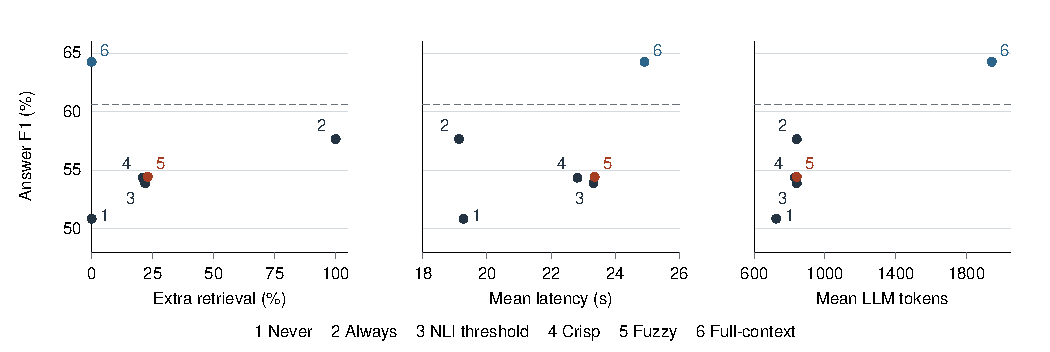
\includegraphics[width=.98\textwidth]{quality_cost.pdf}
\caption{Held-out answer F1 against test re-retrieval rate and live mean costs. The dashed line marks the A/B Oracle F1. Re-retrieval rate uses the full test set. The latency and token axes use 32 shared questions per policy.}
\label{fig:quality-cost}
\end{figure*}


\subsection{Quality, Selection, and Cost}
Table~\ref{tab:quality} reports quality and triggering. Fuzzy improved on Never by 3.576 answer-F1 points, with a paired 95\% interval of $[2.265,4.914]$ points. It selected 56 of the 123 questions on which B improved over A and activated extra retrieval on 230 of the 1,000 questions. Always reached 57.66\% F1 and Fuzzy reached 54.42\%. The A/B Oracle reached 60.61\%, indicating 9.758 points of paired headroom over Never. Table~\ref{tab:paired} lists all five paired contrasts. As shown in Table~\ref{tab:changes}, selecting B for every question improved 123 results and harmed 50. Fuzzy improved 56 and harmed 17 relative to Never.

Fuzzy's mean latency was 23.36~s against 19.13~s for Always (Table~\ref{tab:cost}). The gated path adds the cost of first-round generation and NLI before any second-round generation. Full-context attained the highest answer F1, 64.27\%, exceeding Fuzzy by 9.841 points ($[7.098,12.614]$). Its mean latency was 24.91~s, and its average LLM input had 1,916.75 tokens versus 810.19 for Fuzzy. Figure~\ref{fig:quality-cost} shows these operating points. Every Full-context prompt in this comparison fit the context limit.

\subsection{Fuzzy Versus Crisp and Signal Ablations}
Fuzzy's answer-F1 difference from crisp was 0.064 points ($[-0.365,0.517]$). The policies shared the 20\% dev target and had held-out trigger rates of 23.0\% and 20.9\%. They both triggered on 193 questions, with 37 Fuzzy-only and 16 crisp-only triggers. The interval allows small effects in either direction. The unequal held-out rates further limit attribution of a quality difference to the form of the rule. Fuzzy's F1 exceeded that of NLI-only by 0.531 points ($[0.155,0.994]$). That comparison also changes the input signals.

For the no-NLI ablation, we hold the risk at the midpoint of the locked Fuzzy anchors, which sets its high-risk membership to .5. The no-bridge ablation uses $s=h(r)$. Both apply the original boundary. Removing NLI raised recall from .455 to .813 with an increase in the trigger rate from 23.0\% to 66.0\%. Precision fell from .243 to .152. Removing the bridge feature reduced recall to .382 and answer F1 to 53.79\%, with a 20.7\% trigger rate. Table~\ref{tab:gate} provides the selection metrics at the resulting operating points.

\subsection{Exploratory Error Analysis and Limitations}
The full-set diagnostic found 67 missed improved questions. B added a gold paragraph for 53 of them. Among the 17 harmful Fuzzy triggers, B added a gold paragraph for three. After observing aggregate results, we drew an exploratory sample of 22 distinct questions by stable hash order. It contained five missed improvements, five harmful triggers and four candidates each for missing-hop, wrong-citation and joint-support inspection.

For a question about \emph{The Rum Diary}, A cited the film paragraph and supplied the director for a question about a producer ($p_\mathrm{entail}=.9442$). B retrieved the producer's paragraph and supplied the gold answer. In a wrong-citation case, the cited Hong Kong films supported the output's genre wording while the question referred to an actress from \emph{Moana}. Entailment was .9946. In the Great Fire of London example, the two cited passages linked the church to the fire and supplied the number 87. The selector retained only the sentence stating the number. These cases show differences among textual overlap, multi-hop support and the final sentence set. One harmful trigger also illustrates answer-length sensitivity. Adding \textit{due to} before a correct injury span reduced token F1 from 1.0 to .667.

The held-out study evaluates one answer model, one NLI checkpoint and bridge questions from a single public split. Gate differences can reflect changes in test trigger rates after dev calibration. The lexical bridge feature can miss title variants, and official token overlap can penalize semantically equivalent outputs. The cost estimates describe one hardware and serving configuration on a 32-question sample. Case observations are qualitative readings without independent human adjudication.
